The next step after feature extraction is feature matching. As explained in section~\ref{sec:feature-extraction}, we will get a set of key points and their descriptors for each image. The matching process uses the descriptor information to find out the corresponding matching points in the images. All the points in one image are compared to all the points in other image and best matched point is identified. The nearest-neighborhood based algorithms are basically used for feature matching and since those methods are slower, we have to optimize to get the faster matching. The first section of this chapter gives exhaustive \emph{k-nearest-neighborhood (kNN)} method, then we discuss \emph{approximate nearest neighborhood (ANN)} method in the following section. The fine-tuning of the matching points has been described in last two sections.    

\section{kNN Matching}
\label{sec:knn-matching}
 The k-nearest neighbor (kNN) search problem is widely used in classification problem. If we have a set $P$ of reference points $P=\left\{ p_1,p_2, p_3,...,p_m \right\}$ in $d$-dimensional space, and suppose $q$ be the query point defined in the same space, then kNN search problem determines the $k$ points closest to $q$ among $P$ as shown in figure~\ref{fig:knn-search}.  

\begin{figure}%
\centering
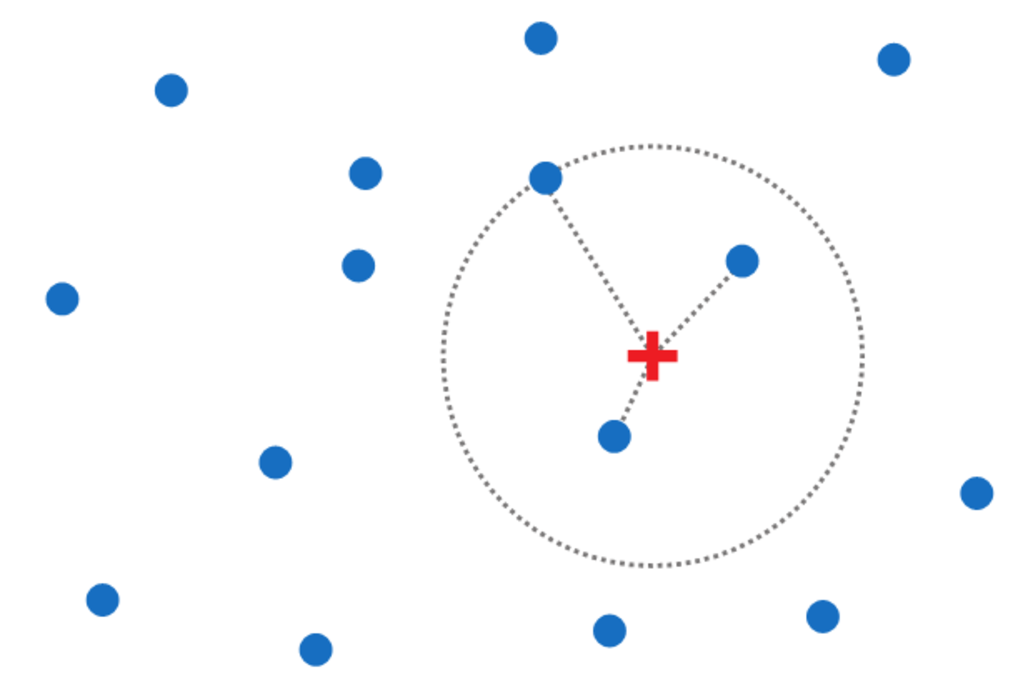
\includegraphics[width=0.6\columnwidth]{2.mainmatter/2.Methodology/figures/Knn}%
\caption[kNN Search]{kNN search problem with k=3. \imgsrc{(Image source: Garcia et al.~\cite{Garcia:10})}}%
\label{fig:knn-search}%
\end{figure}

\section{ANN Matching}
\label{section:ann-matching}
Since, we have high dimensional feature vector \footnote{Each SIFT point has 128 features while a SURF point has 64 features}, and obviously we will have a lot of key points. So, in image stitching problems, exhaustive matching process (such as kNN) is very slow, we select an alternative approximate nearest neighborhood matching i.e. \emph{ANN Matching} where priority-search is carried out on hierarchical k-means trees~\cite{muja:09}. The nearest points need not necessarily be the actual matched points, further tests are necessary to increase matching accuracy (e.g. Ratio Test, Symmetry Test).\\

\noindent The ANN algorithms can be orders of magnitude faster than kNN search, and provides nearest optimal accuracy~\cite{muja:09}. 


\section{Removing False Matches}
The nearest neighborhood based feature matching techniques mentioned above might contain a lot of false matches. Before we go for estimation of transformation parameters, we have to remove those false matches. This section describes the two effective methods to remove false matches: \emph{Ratio Test} and \emph{Symmetry} Test~\cite{Laganière:11}. 
\subsection{Ratio Test}
\label{sec:ratio-test}
For kNN search, if we set $k=2$, the matching finds the two nearest points. The ratio test is based upon the ratio of distances of the two nearest points. Suppose $d_1$ and $d_2$ ($d_1<d_2$) be the distances of a point to its nearest matched points, and a we define a threshold $T$. Then, we reject the points as false matches which satisfy the following condition:
\begin{equation}
\frac{d_1}{d_2}>T
\label{eq:ratio-test}
\end{equation}
If two nearest points are almost same distance, the ratio tend to be higher which implies the false matches, so ratio test confirms the nearest point should be very near and other point should be far. To what extent we remove the points depends upon the threshold $T$ selected i.e. higher the threshold, larger number of matches. Generally, we select $T$=0.8 i.e. if the distance ratio between the two nearest points is greater than 0.8, then ratio test discards that matching pair. Generally, we get more accurate matches by decreasing threshold value; but this is not always true. In some cases, if the image contains similar points (i.e. $d_1 \approx d_2$) in different locations, then ratio $\frac{d_1}{d_2}$ for a match might be higher than threshold ($T$) and the match is discarded.


\subsection{Symmetry Test}
\label{sec:symmetry-test}
In symmetry test, we compute the matches between the images in both direction and select the matches which pass the symmetry test i.e. any matching pair should be symmetrically valid to be accurate match; otherwise the match is discarded as false match. This is very effective test to identify the false matches and we generally prefer to carry out this test after ratio test.\\

\noindent Suppose, a key-point $p_1$ in the first image gets a matched point $p_1'$ in the second image, then match pair \{$p_1$, $p_1'$\} to be an accurate match, the key-point $p_1'$ in the second image should have matched point $p_1$ in the first image. If $p_1'$ gets other key-point as matched point then \emph{Symmetry Test} discards the matched pair \{$p_1$, $p_1'$\}. This test is simple to implement and we do not need any parameters to perform this test.

\newpage
\section{Experimental Results}
\label{sec:feature-matching-experimental-result}
In this section, I will evaluate the feature matching methods in term of computational complexity. Section~\ref{sec:SIFT-SURF} compares SIFT and SURF features matching and section~\ref{sec:kNN-ANN} compares the nearest neighborhood methods (i.e. kNN and ANN) for feature matching. 

\subsection{SIFT versus SURF}
\label{sec:SIFT-SURF}
To carry out the evaluation between SIFT and SURF, I varied the number of feature points in first image by changing threshold values while the number of feature points in the second image made fixed with constant threshold value. The chart presented in figure~\ref{fig:chart:SIFT-SURF} shows that SURF is quite faster than SIFT. The computational cost for SIFT increases drastically as the number of points increases. I used exhaustive kNN matching to match the features.
\begin{figure}[H]%
\centering
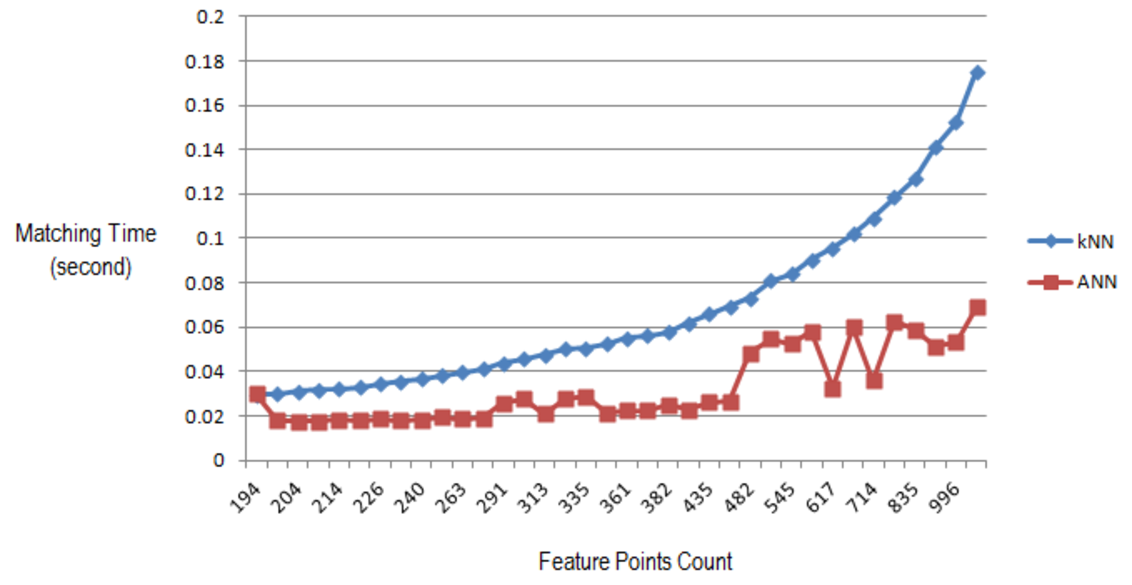
\includegraphics[width=1.2\columnwidth]{2.mainmatter/2.Methodology/figures/SIFT-SURF}%
\caption[Comparison of SIFT and SURF]{Comparison of SIFT and SURF: Feature points versus computational time}%
\label{fig:chart:SIFT-SURF}%
\end{figure}

\noindent SIFT is more accurate because of its high dimensional features, its high computational time is the main drawback making it inappropriate for real time or user-centered applications like medical software. I have chosen SURF method because it is faster and still it gives accurate matches. 

\subsection{kNN versus ANN}
\label{sec:kNN-ANN}
In this section, I will present experimental results on kNN and ANN matching methods for SURF features (64 dimensions) which is presented in graph shown in figure~\ref{fig:knn-ann}. The graph clearly shows that ANN matching always faster than kNN. kNN matching is showing exponential increase in computational complexity when key-points are increased which implies that kNN becomes expensive for large key-points. In practice, we have larger number of feature points to be matched, so ANN matching is preferred to kNN.

\begin{figure}[H]%
\centering
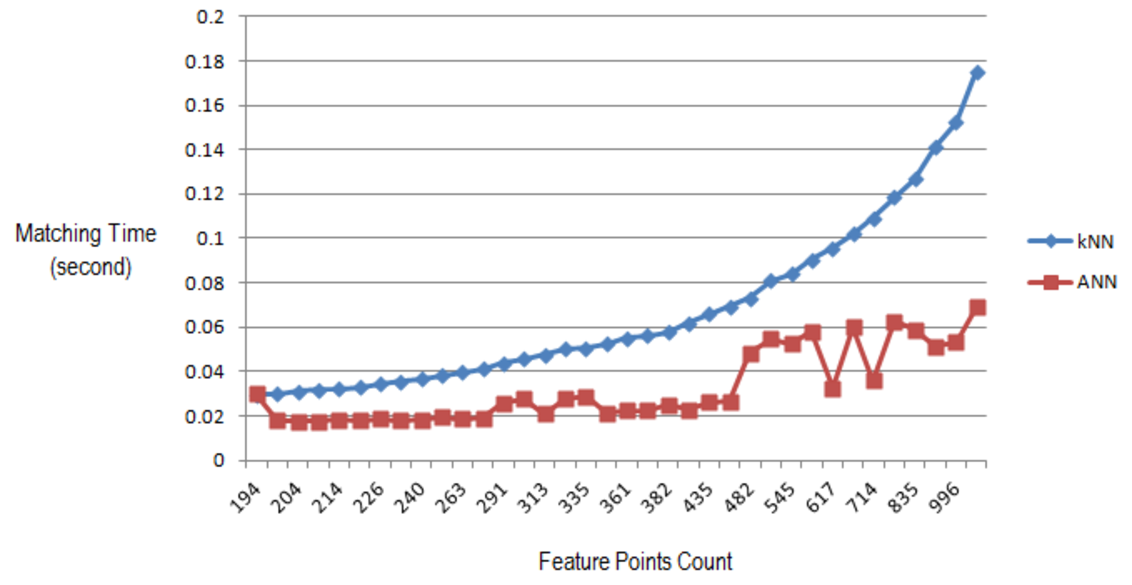
\includegraphics[width=1.3\columnwidth]{2.mainmatter/2.Methodology/figures/kNN-ANN}%
\caption[Comparison of kNN and ANN]{Comparison of kNN and ANN: Feature points vs. matching time}%
\label{fig:knn-ann}% 
\end{figure}

\subsection{Getting Accurate Matches}
\label{sec:accurate-matches}
The nearest neighborhood method just gives the closest point as the matching point which is not necessarily the true match. So, we have to implement tests to remove the false matches identified by nearest neighborhood method. In this section, I implemented some tests to increase the accurate matches by identifying possible false matches. The increment of accurate matches helps to get more accurate transformation model (i.e. \emph{homography}).\\ 

\noindent I have implemented \emph{Ratio} (section~\ref{sec:ratio-test}) and \emph{Symmetry} (section~\ref{sec:symmetry-test}) tests and presented the results in graphical form as shown in figure~\ref{fig:accurate-matches}. The ANN matching resulted 1295 matches (figure~\ref{fig:matches-nn}) , then a significant number of inaccurate matches (1118 matches) are removed by Ratio test (figure~\ref{fig:ratio-test}). For remaining 177 matches, I carried out Symmetry test, which again removed 80 inaccurate matches to get 97 best matches as shown in figure~\ref{fig:symmetry-test}. Although these tests removed significant number of inaccurate matches, the obtained best matches are not 100\% accurate which we can be clearly seen in figure~\ref{fig:symmetry-test}. The remaining inaccurate matches can be identified as outliers by robust estimation methods discussed in the next chapter.


\begin{figure}[H]%
\begin{center}
\subfloat[Nearest neighborhood matches]{\label{fig:matches-nn} 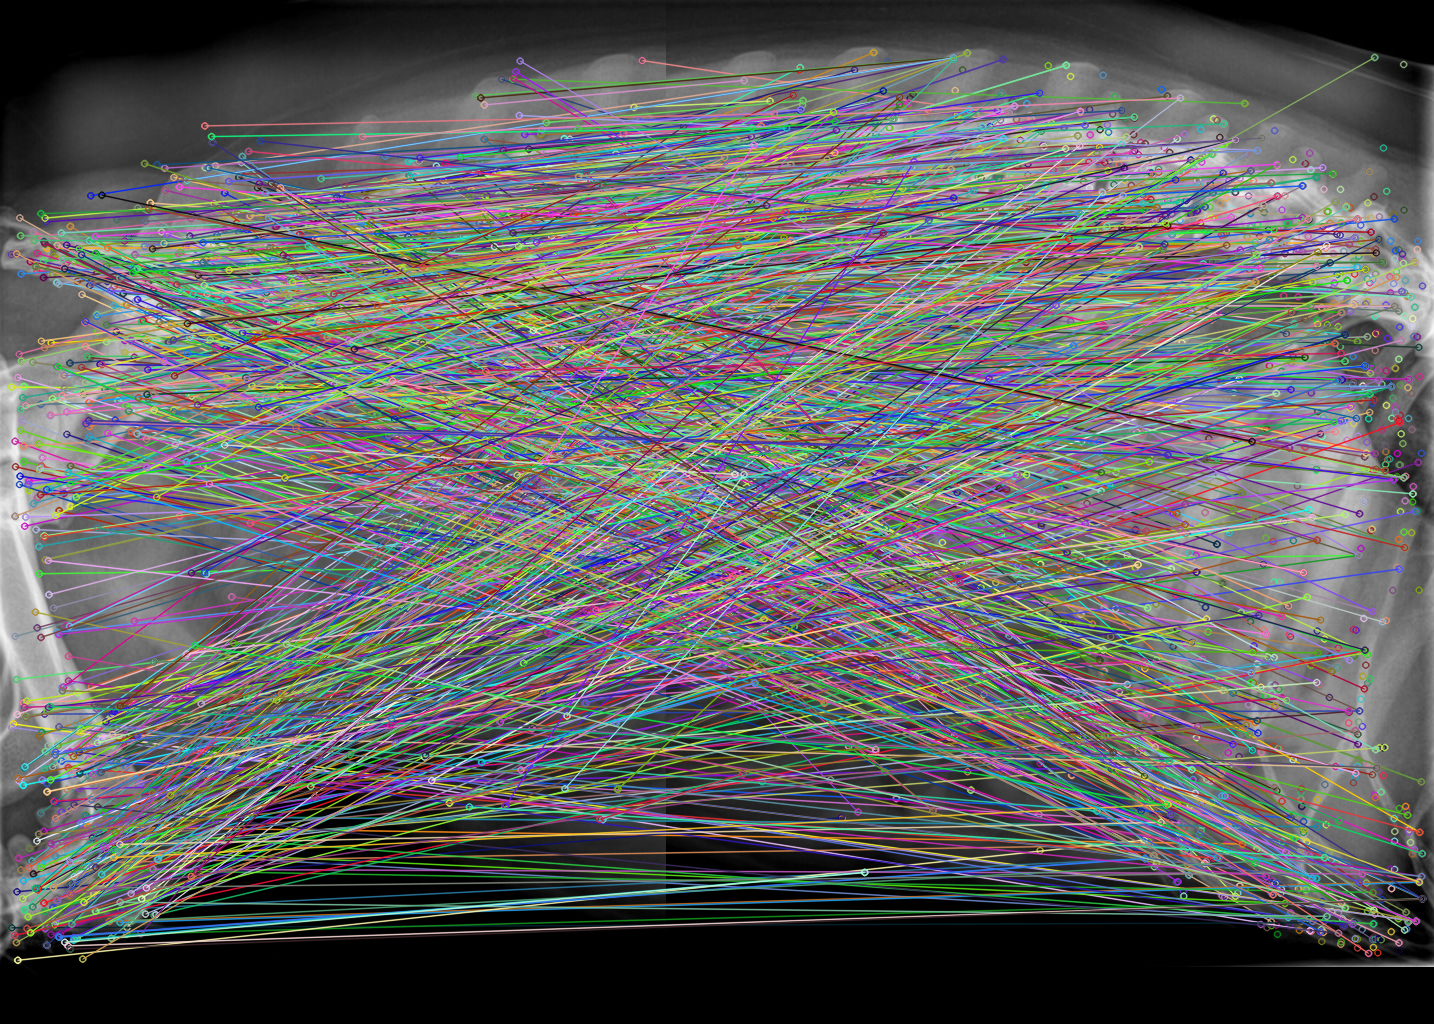
\includegraphics[width= 0.70\columnwidth]{2.mainmatter/2.Methodology/figures/matches}} \hspace{1mm}
\subfloat[Ratio Test] {\label{fig:ratio-test} 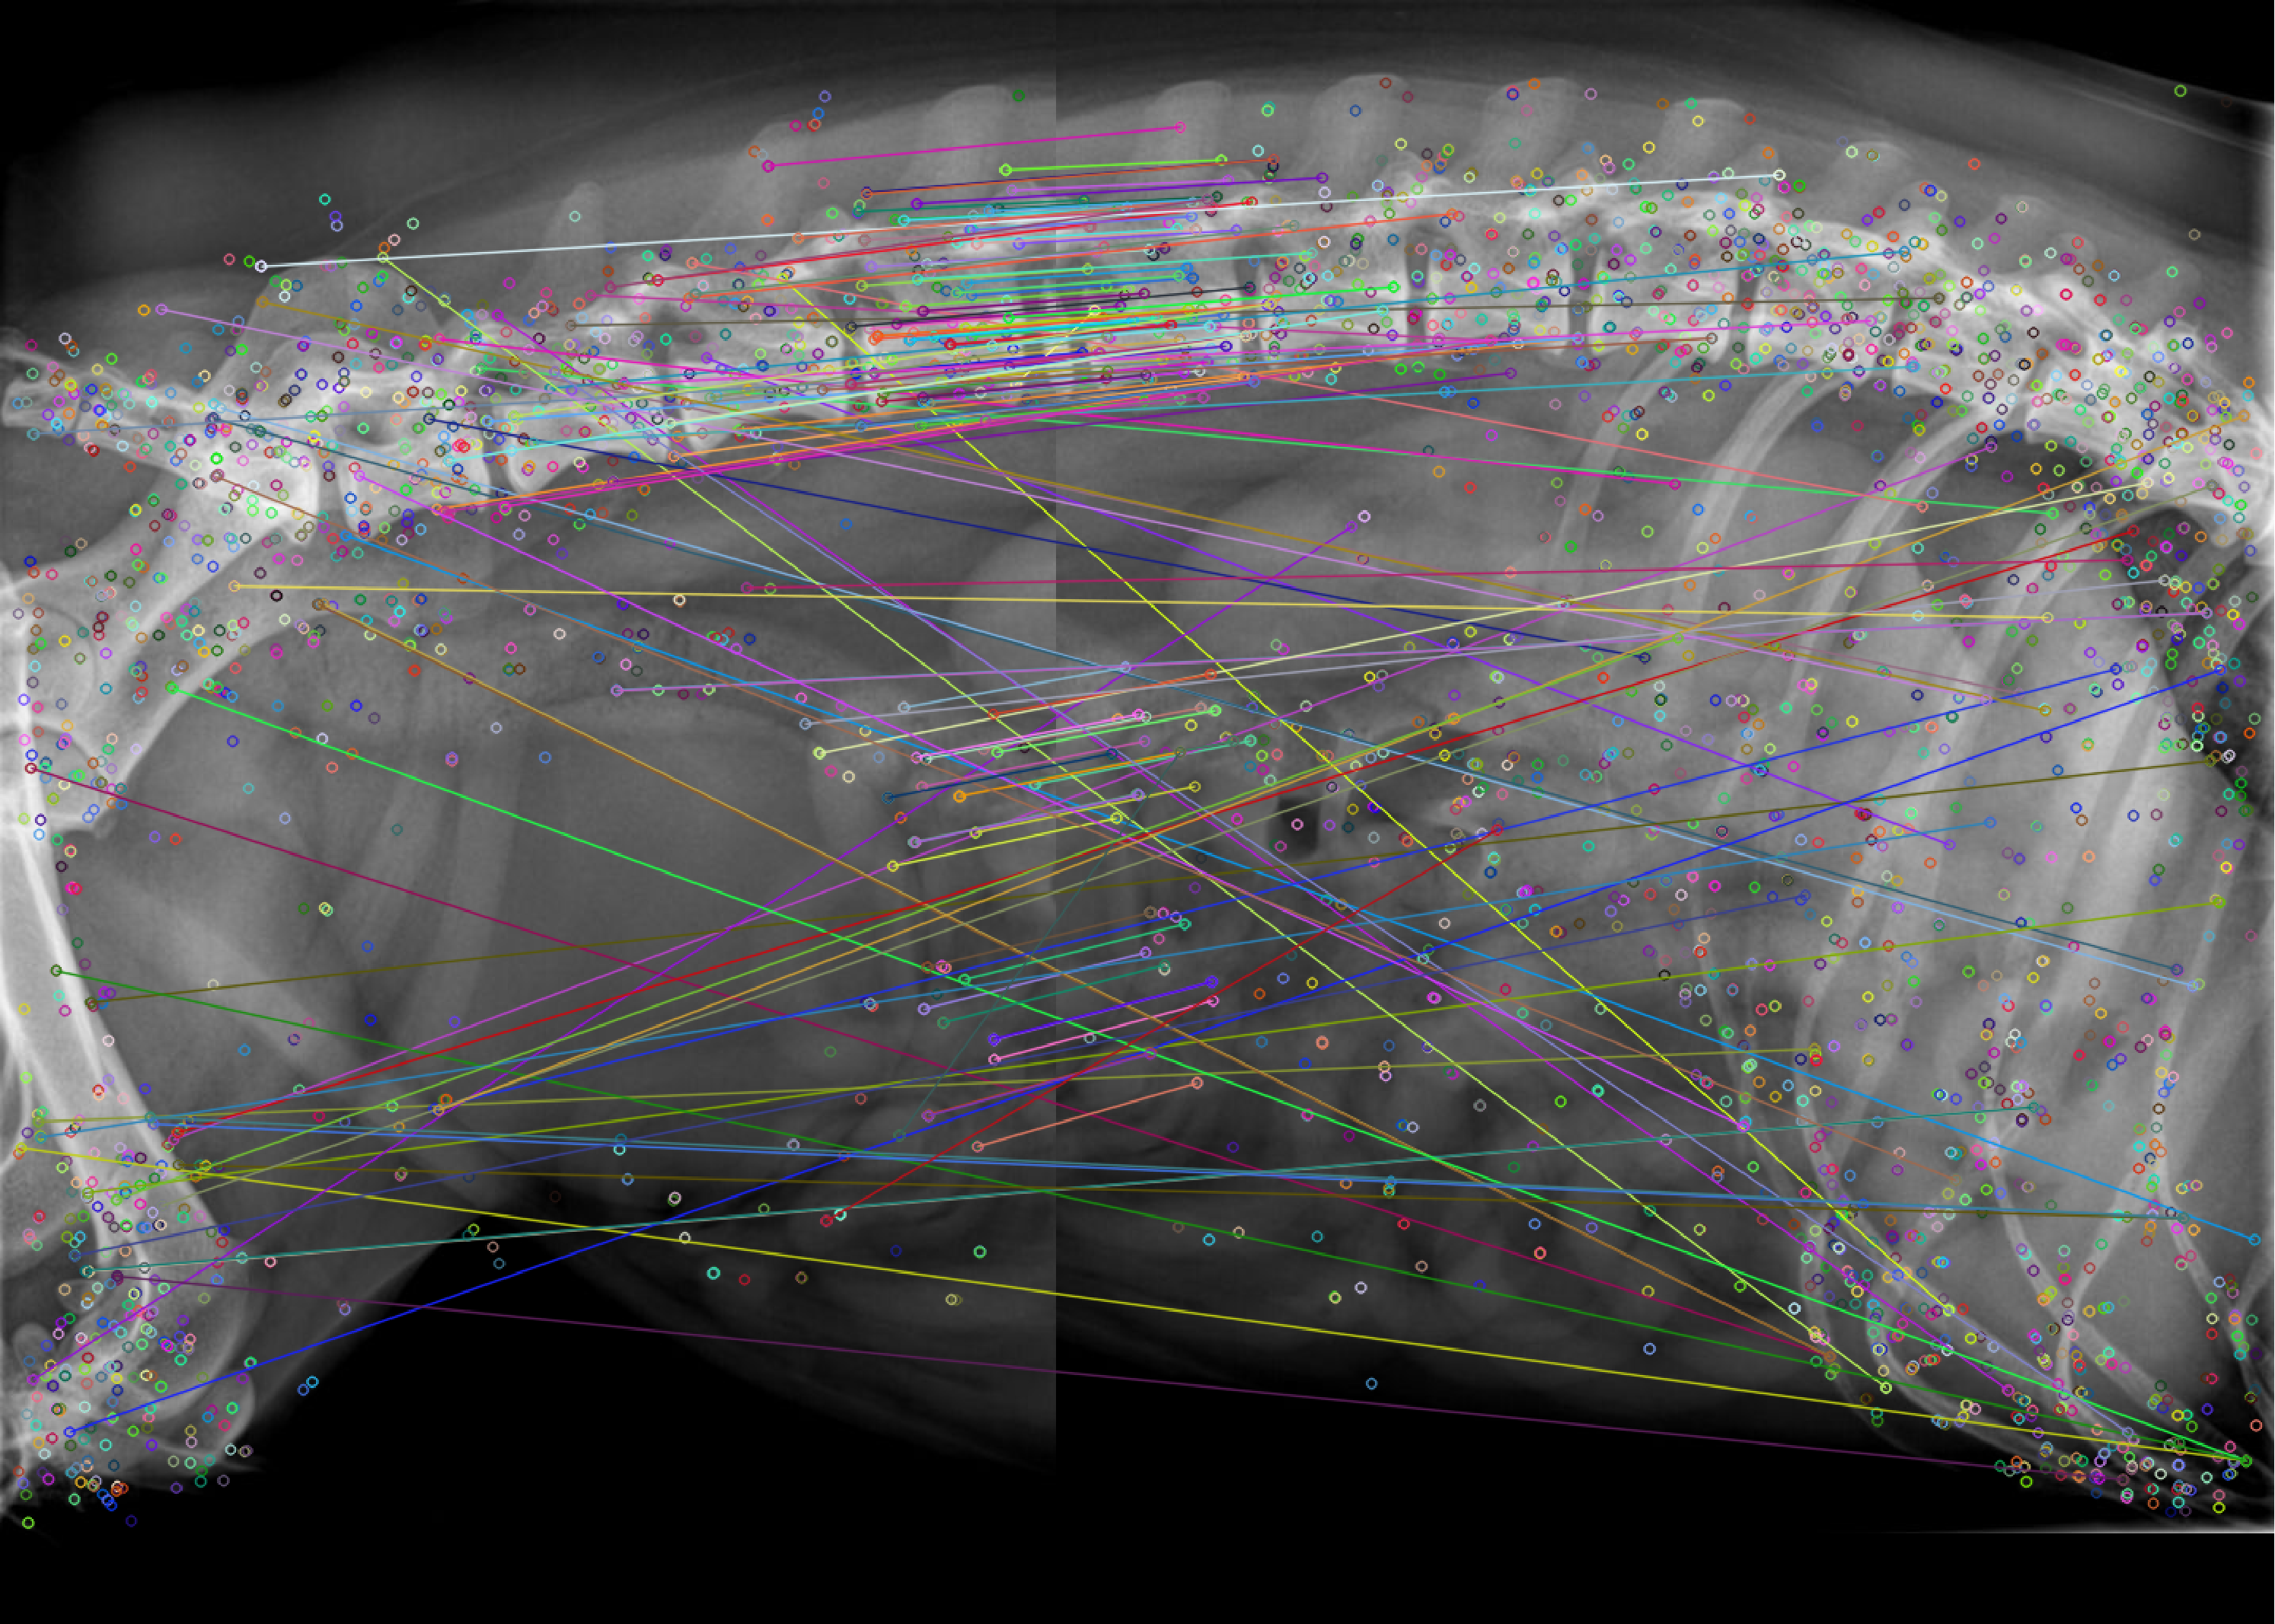
\includegraphics[width= 0.70\columnwidth]{2.mainmatter/2.Methodology/figures/ratio-test}}\quad
\subfloat[Symmetry Test] {\label{fig:symmetry-test} 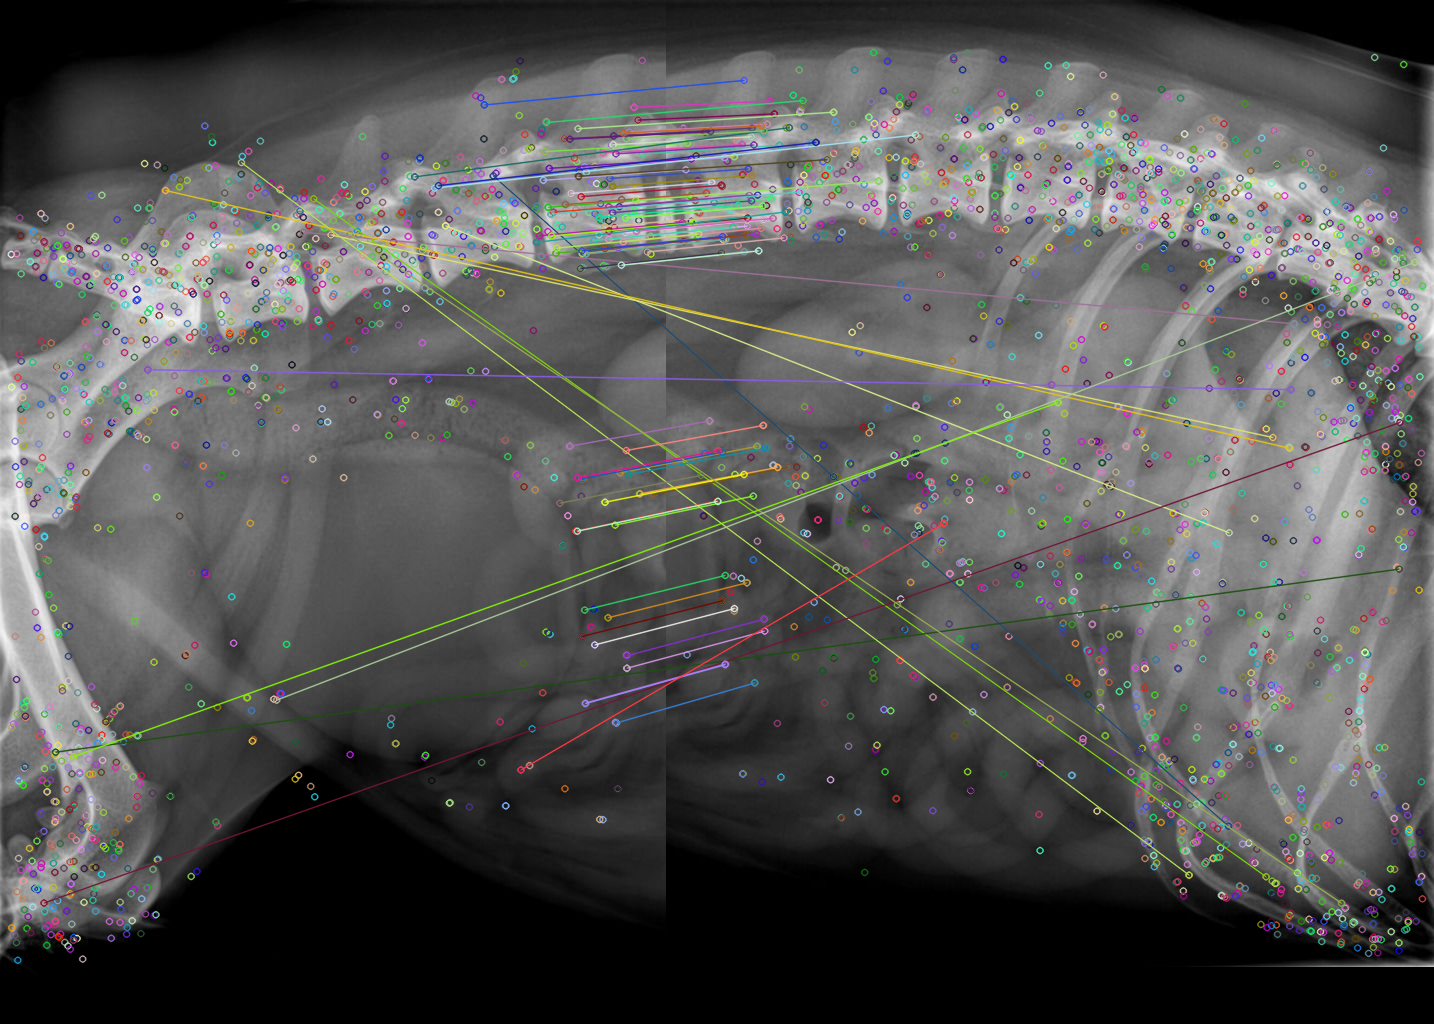
\includegraphics[width= 0.70\columnwidth]{2.mainmatter/2.Methodology/figures/symmetry-test}}
\caption[Steps of Getting Best Matches]{Steps of getting best matches:~\subref{fig:matches-nn} a lot of matches found using NN method~\subref{fig:ratio-test} Ratio test removed a significant number of false matches.~\subref{fig:symmetry-test} The false matches from ratio test are further removed by symmetry test.}%
\label{fig:accurate-matches}%
\end{center}
\end{figure}



